\section{Particiones de enteros}

\begin{defn}
    Dado un número entero no negativo $n$, denotamos por $p(n)$ a la cantidad de maneras de expresar $n$ como la suma de enteros positivos. Cada una de dichas maneras es una \ul{partición} de $n$ y si $\prop$ es una propiedad definida por un conjunto de restricciones para las particiones, denotamos por $p(n|\prop)$ a la cantidad de particiones de $n$ que tienen la propiedad $\prop$.
    
    Por ejemplo,
    
    \begin{gather*}
        p(5) = 7 \\
        p(10) = 42 \\
        p(100) = 190569292
    \end{gather*}
\end{defn}

Este concepto es bastante útil en por ejemplo esta clase de problemas:

\begin{prob}
    ¿De cuántas maneras se puede cambiar un billete de $100$ usando billetes de $50$, $20$, $10$ y $5$?:
    
    Esto equivale a contar la cantidad de maneras de expresar el número $100$ como suma de los números $50$, $20$, $10$ y $5$. En este caso, no es relevante el orden de los sumandos, cada sumando puede estar repetido e incluso es posble que uno o más de los números no se use. Es decir, se trata de contar las particiones del número 100, sujetas a la restricción debida a las denominaciones de los billetes a usar.
\end{prob}

\begin{notn}
    Dado un entero positivo $n$, es usual denotar por
    
    \[
    [1^{\alpha_1}2^{\alpha_2} \dots n^{\alpha_n}]
    \]
    
    \noindent a la partición de $n$ en la cual cada $i$ aparece $\alpha_i$ veces. Como es natural, si $\alpha_i=1$, se omite. Por ejemplo, si $n = 5$
    
    \begin{gather*}
        5 \leftrightarrow [5] \\
        4 + 1 \leftrightarrow [1 \ 4] \\
        2 + 2 + 1 \leftrightarrow [1 \ 2^2]
    \end{gather*}
    
    También es conveniente escribir las particiones de manera gráfica. Por ejemplo, la partición $[6 \ 5 \ 4^2 \ 2 \ 1^3]$ la graficamos así:
    
    \vspace{5mm}
    
    \begin{figure}
        \centering
        \begin{ferrers}
            \row{6} \row{5} \row{4} \row{4} \row{2} \row{1} \row{1} \row{1}
        \end{ferrers}
        \caption{Diagrama para la partición $[6 \ 5 \ 4^2 \ 2 \ 1^3]$.}
        \label{fig:ferrers1}
    \end{figure}
    
    Es decir, que para cada $i \leq n$ graficamos $\alpha_i$ filas, cada una con $i$ puntos. Esto se conoce como \textit{diagrama de Ferrers} para la partición.
\end{notn}

Estos diagramas son bastante convenientes en una cantidad diversa de problemas. Por ejemplo:

\begin{prob}
    Dados enteros positivos $n, r$, analicemos la partición
    
    \[
    p(n+r|\text{cantidad de partes $= r$})
    \]
    
    ¿Cómo es el diagrama de Ferrers para una partición de este tipo? ¿Cuántas marcas tiene la primera columna?
    
    \begin{marginfigure}
        \centering
        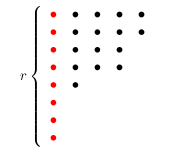
\includegraphics[scale=0.65]{img/ferrers2.png}
        \caption{Diagrama de Ferrers para la partición presentada en el problema. Vemos que la primera columna tiene $r$ puntos (uno para cada parte).}
        \label{fig:ferrers2}
    \end{marginfigure}
    
    Si se elimina la primera columna, queda el diagrama de una partición de $n$, y la partición que queda tiene a lo sumo $r$ partes. Es decir, a cada partición de $n+r$ con $r$ partes, le corresponde una partición de $n$ con a lo sumo $r$ partes.
    
    Ahora, dada una partición de $n$ con a lo sumo $r$ partes. ¿Podremos obtener una partición de $n+r$ con $r$ partes?: Basta con agregar una primera columna con $r$ puntos.
    
    \begin{marginfigure}
        \centering
        \begin{ferrers}
            \row{4} \row{4} \row{3} \row{3} \row{1}
        \end{ferrers}
        \caption{Acá estamos omitiendo la primera columna. Vemos que al agregarle la columna con $r$ puntos, estamos sumando $r$ puntos a la partición de $n$ que ya tenemos, por lo que resulta en $n+r$ puntos en total.}
    \end{marginfigure}
\end{prob}

Este hecho presentado en el problema puede resumirse de la siguiente manera.

\begin{teo}
    Dados enteros positivos $n$ y $r$,
    
    \[
    p(n+r|\text{cantidad de partes de $= r$}) = p(n|\text{cantidad de partes $\leq r$})
    \]
\end{teo}

Otro concepto que es útil para trabajar estos problemas es el de \textit{partición conjugada}. Dada una partición $\lambda$, la partición $\lambda'$ obtenida cambiando filas por columnas en el diagrama de Ferrers $\lambda$, se llama partición \textit{conjugada} de $\lambda$.

\begin{ejer}
    Dados enteros positivos $n$ y $m$, demuestra que la función dada por $\lambda \rightarrow \lambda'$ es una biyección entre el conjunto de las particiones de $n$ con parte máxima $m$ y el conjunto de las particiones de $n$ con $m$ partes. ¿Cómo se escribe esto con la notación $p(n|\prop)$?
\end{ejer}

\begin{proof}[Solución]
    La función $\lambda \rightarrow \lambda'$ es tal que las filas de $\lambda$ son las columnas de $\lambda'$. Entonces si $\lambda$ tiene $m$ partes, su primera columna tiene $m$ puntos, por lo tanto la primera fila de $\lambda'$ tiene $m$ puntos. De esta forma, la función $\lambda \rightarrow \lambda'$ es una biyección del conjunto de las partes de $n$ con parte máxima $m$ al conjunto de las partes de $n$ con $m$ partes. Luego
    
    \[
    p(n|\text{parte máxima = $m$}) = p(n|\text{$\#$ partes = $m$})
    \]
\end{proof}

Decimos que una partición $\lambda$ es \textit{autoconjugada} si $\lambda = \lambda'$. ¿Qué se puede decir de las particiones autoconjugadas a partir de su diagrama de Ferrers?

\begin{figure}
    \centering
    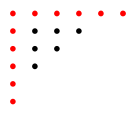
\includegraphics[scale=0.65]{img/ferrers3.png}
    \caption{Diagrama de Ferrers para la situación presentada.}
    \label{fig:ferrers3}
\end{figure}

Observemos el número total de puntos en la primera fila y primera columna. Si se eliminan esas marcas, ¿qué queda?: Como tienen la misma cantidad de puntos, digamos $k$, y como tienen un punto en común, el número total de puntos removidos es $2k-1$ (el cual es un número impar). De la misma forma, al remover las primera fila y columna en el nuevo diagrama, tendremos otra cantidad impar de puntos removidos, digamos $2l-1$. Haciendo esto de forma iterativa, encontraremos una nueva partición de $n$ donde cada una de sus partes es de tamaño impar y son todas distintas entre sí.

Equivalentemente, si tenemos una partición donde cada parte es de tamaño par y distintas entre sí, si cada parte es mayor que $1$ podemos formar una fila y una columna de tamaño, digamos $k+1$, tales que comparten un punto entre sí. Procediendo de manera iterativa, como cada una de las partes es distinta e impar, la partición resultante tendrá la característica de que al intercambiar las filas por columnas, cada una de ellas tendrá la misma cantidad de puntos en cada parte. De esta manera podemos enunciar el siguiente teorema:

\begin{teo}
    Dado un entero positivo $n$,
    
    \[
    p(n|\text{partes distintas e impares}) = p(n|autoconjugada)
    \]
\end{teo}

Sin embargo, calcular $p(n)$ no resulta algo tan trivial. Los métodos para encontrar $p(n)$ los encontraremos en las fórmulas generadoras y las sumas formales infinitas: Dados enteros positivos $n$ y $m$, analicemos

\[
a_n = p(n|\text{cada parte $= m$})
\]

Solamente podremos encontrar dichas particiones si $n$ es un múltiplo de $m$. Entonces $n$ es una partición $n = m + m + m + \dots$. Es decir,

\[
a_n =
\begin{cases}
    1 \quad \text{si $m$ divide a $n$} \\
    0 \quad \text{en otro caso}
\end{cases}
\]

Entonces definiendo $a_0 = 1$, tenemos

\[
\sumtoinfty{n=0}{a_nx^n} = 1 + x^m + x^{2m} + \dots
\]

Por lo tanto $f_m(x) = (1-x^m)^{-1}$ es una fórmula generadora para $p(n|\text{cada parte $= m$})$, con $n \geq 0$. Sea ahora un entero $r$ y definamos

\begin{gather*}
    b_n = p(n| \text{cada parte $=r$}) \\
    c_n = p(n| \text{cada parte $= m$ o $= r$})
\end{gather*}

¿Cómo podríamos calcular $c_n$? Observamos que $c_n$ es la cantidad de maneras de escribir $n$ como suma de $t$ y $n-t$ tales que $t$ está partido en partes de tamaño $m$ y $n-t$ está partido en partes de tamaño $r$. Entonces

\[
c_n = a_0b_n + a_1b_{n+1} + \dots + a_nb_0
\]

Y por definición de producto de sumas formales infinitas, la sucesión de los $c_n$ está generada por

\[
f_m(x)f_r(x) = (1-x^m)^{-1}(1-x^r)^{-1}
\]

De esta forma, podemos resolver problemas del siguiente tipo:

\begin{prob}
    ¿De cuántas maneras se puede escribir el número $10$ como sumas que sólo usan los números $2$ y $3$?: Basta con ver el coeficiente de $x^{10}$ en
    
    \[
    (1-x^2)^{-1}(1-x^3)^{-1}
    \]
    
    En cuyo caso obtenemos $2$.
\end{prob}

De forma análoga podemos concluir que para calcular $p(n|\text{cada parte $=i, j$ ó $k$})$ debemos hayar el coeficiente de $x^n$ en el producto 

\[
(1-x^i)^{-1}(1-x^j)^{-1}(1-x^k)^{-1}
\]

Usando esta idea podemos concluir que el coeficiente de $x^n$ en el producto

\[
(1-x^1)^{-1}(1-x^2)^{-1}\dots(1-x^n)^{-1}
\]

\noindent es la cantidad de particiones de $n$ en las que cada parte es de tamaño $1$, o $2$, \dots, o $n$. Es decir \textit{todas} las particiones de $n$. Conclusión: una fórmula generadora para $p(n)$ es

\[
P(x) = \prod_{i=1}^{\infty} (1-x^i)^{-1}
\]

\subsection{Calcularndo $p(n)$}

Los métodos expuestos anteriormente nos permiten escribir funciones generadoras para los números de particiones tales que se satisfacen ciertas restricciones: ¿Qué ocurre si cada parte aparece a lo sumo $k$ veces? En ese caso tendremos un factor de la forma

\[
(1 + x^i + x^{2i} + \dots + x^{ki}), \quad \text{para cada tamaño $i$}
\]

\noindent en lugar de la suma formal infinita. En consecuencia una fórmula generadora sería

\[
\prod_{i=1}^{\infty} (1 + x^i + x^{2i} + \dots + x^{ki}) = \prod_{i=1}^{\infty} \frac{1 - x^{(k+1)i}}{1-x^i}
\]

En particular, si tenemos $k=1$ entonces esto nos da

\[
p(n | \text{partes son distintas}) = (1+x)(1+x^2)(1+x^3)\dots
\]

Otras fórmulas generadoras sencillas (y fácilmente verificables) son

\begin{gather*}
    p(n | \text{partes con tamaño impar}) = \frac{1}{(1-x)(1-x^3)(1-x^5)\dots} \\
    p(n | \text{partes con tamaño par}) = \frac{1}{(1-x^2)(1-x^4)(1-x^6)\dots} \\
    p(n | \text{partes con tamaño $\leq m$}) = \frac{1}{(1-x)(1-x^2)\dots(1-x^m)}
\end{gather*}

Observemos que a partir de

\[
(1+x)(1+x^2)(1+x^3)\dots
\]

\noindent al multiplicar y dividir por $(1-x^i)$ con $i = 1, 2, \dots$ nos queda que

\[
\frac{(1-x^2)(1-x^4)(1-x^6) \dots}{(1-x)(1-x^2)(1-x^3) \dots}  = \frac{1}{(1-x)(1-x^3)(1-x^5) \dots}
\]

En conclusión, para cada $n$, $p(n | \text{partes con tamaño impar})$ y $p(n | \text{partes dinstintas})$ tienen la misma fórmula generadora, por lo que

\[
p(n | \text{partes con tamaño impar}) = p(n | \text{partes distintas})
\]

Ahora, recordemos que la fórmula

\[
P(x) = \prod_{i=1}^{\infty}(1-x^i)^{-1}
\]

\noindent genera la suceción $\{p(n)\}_{n=0}^{\infty}$. Si multiplicamos esto por

\[
Q(x) = \prod_{i=1}^{\infty} (1-x^i)
\]

\noindent el resultado es 1, entonces el coeficiente de $x^n$ en $P(x)Q(x)$ para $n \geq 1$ es cero, por lo que se cumple

\[
q_0P(n) + q_1P(n-1) + \dots + q_n = 0
\]

Es decir, que si conocemos los $q_n$'s podremos obtener una relación recursiva para $p(n)$, así que analicemos $Q(x)$. Calculando los primeros términos se obtiene

\[
1 - x - x^2 + x^5 + x^7 - x^{12} - x^{15} + x^{22} + x^{26} - \dots
\]

Aparentemente la mayoría de los coeficientes son cero, mientras que el resto es $1$ ó $-1$. Para ver esto claramente, primero recordemos el producto

\[
p(n | \text{partes son distintas}) = (1+x)(1+x^2)(1+x^3)\dots
\]

En este caso, la partición $7 = 1 + 2 + 4$ corresponde al término $x \times x^2 \times x^4$ y suma $1$ al coeficiente de $x^7$. Consideremos ahora el mismo producto, pero cambiando los signos. Entonces tendremos

\[
Q(x) = \prod_{i=1}^{\infty} (1-x^i) = (1-x)(1-x^2)(1-x^3)\dots
\]

En este caso, la partición $7 = 1 + 2 + 4$ corresponde al término $(-x) \times (-x)^2 \times (-x)^4$ y suma $-1$ al coeficiente de $x^7$. Por lo tanto cada partición de $n$ con partes distintas suma $(-1)^d$ al coeficiente de $x^n$, donde $d$ es la cantidad de partes. Y en general, cada partición de $n$ con una cantidad par de partes distintas suma $1$ a $q_n$, y cada partición de $n$ con una cantidad impar de partes distintas suma $-1$ a $q_n$. Por lo tanto si denotamos por

\begin{gather*}
    e_n = p(n | \text{partes distintas y $\#$ partes par}) \\
    o_n = p(n | \text{partes distintas y $\#$ partes impar})
\end{gather*}

Entonces $q_n = e_n - o_n$. Por lo tanto $q_n = 0$ si $e_n = o_n$.

Analicemos los casos en que $q_n \neq 0$: Para cada partición $\lambda$ con partes distintas, definamos una partición $\lambda'$ tal que la correspondencia será biyectiva en la mayoría de los casos, y para el resto la biyectividad fallará. Denotemos también por $s(\lambda)$ a la parte más pequeña de $\lambda$, y si $\lambda$ tiene $m$ partes, enumeraremos las filas en su diagrama de Ferrers de arriba hacia abajo. Si para cada $i < m$ la fila $i$ tiene exactamente un punto más que la fila $i+1$, definimos $t(\lambda) = m$; en caso contrario, $t(\lambda)$ es el mínimo $i$ tal que la fila $i$ \textbf{no} tiene exactamente un punto más que la fila $i+1$.

\begin{figure}
    \centering
    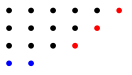
\includegraphics[scale=0.65]{img/ferrers4.png}
    \caption{En este ejemplo, $s(\lambda) = 2$ y $t(\lambda) = 3$.}
    \label{fig:ferrers4}
\end{figure}

Para definir la correspondencia $\lambda \rightarrow \lambda'$ consideraremos dos casos. Si $s(\lambda) \leq t(\lambda)$, eliminamos la parte $s(\lambda)$ y cada punto eliminado lo colocaremos al final de cada una de las $s(\lambda)$ filas del diagrama.

\begin{figure}
    \centering
    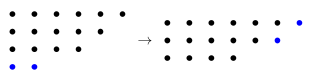
\includegraphics[scale=0.65]{img/ferrers5.png}
    \caption{Vemos aquí que los puntos azules de $\lambda$ se colocan al final de las 2 primeras filas de $\lambda'$.}
    \label{fig:ferrers5}
\end{figure}

Si $s(\lambda) > t(\lambda)$ eliminamos el último punto de cada una de las primeras $t(\lambda)$ y con ellos formamos una nueva última fila.

\begin{figure}
    \centering
    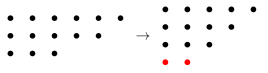
\includegraphics[scale=0.65]{img/ferrers6.png}
    \caption{Los puntos rojos de $\lambda'$ se corresponden con los últimos puntos de las primeras $t(\lambda)$ filas de $\lambda$.}
    \label{fig:ferrers6}
\end{figure}

Resaltamos que la cantidad de partes de $\lambda$ y $\lambda'$ difieren en $1$, por lo que a una partición contada por $e_n$, le corresponde una partición contada por $o_n$ y viceversa. Esta es \textbf{casi} una correspondencia biyectiva, pero ¿cuáles son las excepciones? En el primer caso, si $s(\lambda) = t(\lambda)$ y los puntos correspondientes se solapan, la operación \textbf{no} produce el diagrama de una partición.

\begin{figure}
    \centering
    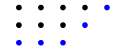
\includegraphics[scale=0.65]{img/ferrers7.png}
    \caption{Vemos que los puntos se solapan.}
    \label{fig:ferrers7}
\end{figure}

Para este caso, $s(\lambda) = m$ y

\[
n = m + (m+1) + (m+1) + \dots + (m+m-1) = \frac{m(3m-1)}{2}
\]

En el segundo caso, si los puntos correspondientes se solapan y $s(\lambda) = m+1$, entonces $\lambda'$ tiene las últimas dos partes iguales.

\begin{figure}
    \centering
    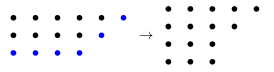
\includegraphics[scale=0.65]{img/ferrers8.png}
    \caption{Vemos nuevamente que los puntos se solapan y $\lambda \rightarrow \lambda'$ no es biyectiva en este caso.}
    \label{fig:ferrers8}
\end{figure}

En este caso tenemos que

\[
n = m + (m+1) + (m+1) + \dots + (m+m) = \frac{m(3m+1)}{2}
\]

Estos resultados los podemos resumir de la siguiente manera:

\begin{teo}
    Si $Q(x)$ está definida por
    
    \[
    Q(x) = \sum_{n=0}^{\infty} q_nx^n = (1-x)(1-x^2)\dots
    \]
    
    \noindent entonces
    
    \[
    q_n = \begin{cases}
              (-1)^m \quad &\text{si $\displaystyle n = \frac{m(3m \pm 1)}{2}$} \\
              0 \quad &\text{en otro caso}
          \end{cases}
    \]
\end{teo}

De esta forma, se obtienen algunos valores no nulos de $q_n$:

\begin{center}
    \begin{tabular}{ccc}
        $m$ & $\displaystyle \frac{m(3m-1)}{2}$ & $\displaystyle \frac{m(3m+1)}{2}$ \\ \toprule
        $1$ & $1$ & $2$ \\
        $2$ & $5$ & $7$ \\
        $3$ & $12$ & $15$ \\
        $4$ & $22$ & $26$ \\
        $5$ & $35$ & $40$ \\
        $6$ & $51$ & $57$
    \end{tabular}
\end{center}

Con lo cual se puede obtener la recurrencia para $p(n)$:

\[
p(n) = p(n-1) + p(n-2) - p(n-5) - p(n-7) + p(n-12) + p(n-15) + \dots
\]